\documentclass[a4paper,11pt,oneside,openany]{memoir}

\usepackage{fontspec}
\usepackage{amsmath} % a pretty standard package to enlarge your inventory of symbols
\usepackage{amssymb} % another common package for symbols
\usepackage[hidelinks]{hyperref} % enables hyperlinks in your document (no worries -- they show up only on the screen. When you print a hard copy, the colored boxes aren't there)
\usepackage{url} % helps typeset URLs properly, typically with the command \url
\usepackage[margin=.75in]{geometry} % page layout
\usepackage{tikz}
\usepackage{tikz-qtree}
\usepackage{wrapfig}
%\usepackage{subcaption}
\usepackage{booktabs} % creates beautiful and professional tables
\usepackage{multicol}
\usepackage{multirow}
\usepackage{textcomp}
\usepackage{expex}
\usepackage{enumitem}
\usepackage{tablefootnote}
\usepackage[calc,english]{datetime2}
\usepackage{suffix}
\usepackage{afterpage}
\usepackage{bookmark}
\usepackage{blindtext}
\usepackage{phonrule}
\usepackage[glosses,indexonlyfirst,nonumberlist,toc,nomain,mcolblock,,nogroupskip]{leipzig}
\usepackage{etoolbox}

\setmainfont{Brill}

%---generic symbols---%
\newcommand{\dao}{$\to$}
\newcommand{\nm}{\symbol{"2205}}
\newcommand{\ra}{\textgreater}
\newcommand{\ipkt}{·}
\newcommand{\til}{\textasciitilde}
\newcommand{\langbr}{⟨}
\newcommand{\rangbr}{⟩}

\newcommand{\ortho}[1]{$\langle$#1$\rangle$}
\newcommand{\bripa}[1]{[#1]}
\newcommand{\phipa}[1]{/#1/}
\newcommand{\eng}[1]{`#1'}

%---IPA---%
%consonants
\newcommand{\bilaf}{ɸ}
\newcommand{\bilav}{β}
\newcommand{\tht}{θ}
\newcommand{\labrox}{ʋ}
\newcommand{\latfric}{ɬ}
\newcommand{\latfrivoic}{ɮ}
\newcommand{\darkl}{ɫ}
\newcommand{\alvr}{ɹ}
\newcommand{\alvrap}{ɾ}
\newcommand{\alvlap}{ɺ}
\newcommand{\esh}{ʃ}
\newcommand{\ezh}{ʒ}
\newcommand{\alvpalesh}{ɕ}
\newcommand{\alvpalezh}{ʑ}
\newcommand{\paljstop}{ɟ}
\newcommand{\paljfric}{ʝ}
\newcommand{\egna}{ɲ}
\newcommand{\retesh}{ʂ}
\newcommand{\retezh}{ʐ}
\newcommand{\retna}{ɳ}
\newcommand{\egh}{ɣ}
\newcommand{\engma}{ŋ}
\newcommand{\vell}{ʟ}
\newcommand{\velr}{ʁ}
\newcommand{\velprox}{ɰ}
\newcommand{\uvux}{χ}
\newcommand{\pharox}{ʕ}
\newcommand{\glotstop}{ʔ}
%vowels
\newcommand{\frno}{ø}
\newcommand{\bari}{ɨ}
\newcommand{\unru}{ɯ}
\newcommand{\unro}{ɤ}
\newcommand{\eps}{ɛ}
\newcommand{\oeps}{œ}
\newcommand{\sche}{ɘ}
\newcommand{\schwa}{ə}
\newcommand{\centruh}{ɜ}
\newcommand{\opno}{ɔ}
\newcommand{\aesh}{æ}
\newcommand{\oesh}{ɶ}
\newcommand{\centra}{ɐ}
\newcommand{\ahoh}{ɒ}
%diacritics and modifiers
\newcommand{\asp}{ʰ}
\newcommand{\lab}{ʷ}
\newcommand{\pal}{ʲ}
\newcommand{\jekt}{ʼ}
\newcommand{\nav}{̃}
\newcommand{\rhot}{˞}
\newcommand{\sylb}{̩}
\newcommand{\vless}{̥}
\newcommand{\upvless}{̊}
\newcommand{\bck}{̠}
\newcommand{\dwnwrd}{̞}
\newcommand{\upwrd}{̝}
\newcommand{\lamino}{̻}
\newcommand{\apico}{̺}
\newcommand{\lowap}{̞}
\newcommand{\prstr}{ˈ}
\newcommand{\scstr}{ˌ}
\newcommand{\tiebar}{͡}
\newcommand{\lgth}{ː}
\newcommand{\linglab}{̼}
%tone letters
\newcommand{\toneH}{˥}
\newcommand{\toneM}{˧}
\newcommand{\toneL}{˩}
\newcommand{\toneMH}{˦}
\newcommand{\toneML}{˨}

\definelingstyle{default}{glstyle=nlevel,numoffset=3em,textoffset=1.5em,exskip=.75ex,belowglpreambleskip=.25ex,aboveglftskip=.25ex,everyglft=\it}

\lingset{lingstyle=default}

\DTMnewdatestyle{eurodate}{%
    \renewcommand{\DTMdisplaydate}[4]{%
        \number##3.\nobreakspace%           day
        \DTMmonthname{##2}\nobreakspace%    month
        \number##1%                         year
    }%
    \renewcommand{\DTMDisplaydate}{\DTMdisplaydate}%
}

\DTMsetdatestyle{eurodate}

%-----DICT COMMANDS------
%------------------------

\makeatletter
\@beginparpenalty=10000
\makeatother

\newcounter{dictwordcount}
\newcounter{definition}

\newenvironment{entrylist}{
    \begin{description}[leftmargin=*]
    }{
    \end{description}
    }

\makeatletter
\newenvironment{simplentry}[1]%
    {%
    \item[#1]\hfill
    \protected@edef\@currentlabelname{#1}%
    \setcounter{definition}{0}%
    \begin{description}[align=right,labelwidth=*,font=\normalfont]
    }{%
    \end{description}
    }%
\makeatother

\makeatletter
\newenvironment{dictentry}[3][]%
    {%
    \item[#2]\ifthenelse{\isempty{#1}}{\hfill}{\:\bripa{#1}\hfill}\\
    {\footnotesize #3}
    \protected@edef\@currentlabelname{#2}%
    \setcounter{definition}{0}%
    \refstepcounter{dictwordcount}%
    \begin{description}[align=right,labelwidth=*,font=\normalfont]
    }{%
    \end{description}
    }%
\makeatother

\newenvironment{entrysublist}{
    \vspace{2ex}
    \item[]\textit{Compounds \& Phrasal Forms}
    \begin{entrylist}
        \small
    }{
    \end{entrylist}
    }

\newcommand{\dictdef}[2][]{\refstepcounter{definition}%
    \item[\thedefinition.] \ifthenelse{\isempty{#1}}{
        #2
    }{
        \textit{#1}\: #2
    }%
    }%

\WithSuffix\newcommand\dictdef*[2][]{%
    \item[] \ifthenelse{\isempty{#1}}{
        #2
    }{
        \textit{#1} #2
    }%
    }

\newcounter{protwordcount}

\makeatletter
\newenvironment{protentry}[1]%
    {%
    \item[\proto{#1}]\hfill
    \protected@edef\@currentlabelname{#1}%
    \setcounter{definition}{0}%
    \refstepcounter{protwordcount}%
    \begin{description}[align=right,labelwidth=*,font=\normalfont]
    }{%
    \end{description}
    }%
\makeatother

%----------------------------
%---------Glossaries---------
%----------------------------

\makenoidxglossaries

\newleipzig{test}{tst}{It's a test!}

\glssetwidest{CABBA}

\makeatletter
\newglossarystyle{fixed-mcols}{%
    \setglossarystyle{alttree}%
    \renewenvironment{theglossary}%
    {%
        \begin{multicols}{3}%
            \def\@gls@prevlevel{-1}%
%           \mbox{}\par
        }%
        {\par\end{multicols}}%
}
\makeatother

%---------------------------
%---------------------------

\newcommand{\enl}[1]{\textit{#1}}
\newcommand{\enlq}[1]{«~#1»}
\newcommand{\proto}[1]{\textit{*#1}}

%---Lang Romanization---%
%\newcommand{\ph}{φ}
%\newcommand{\te}{ϑ}
%\newcommand{\kh}{χ}
\newcommand{\ppa}{π}
\newcommand{\tta}{τ}
\newcommand{\kka}{κ}
\newcommand{\engga}{ng}
\newcommand{\Ppa}{Π}
\newcommand{\Tta}{Τ'}
\newcommand{\Kka}{Κ'}
\newcommand{\Engga}{Ng}

\newcommand{\suph}{$^\textsc{h}$}
\newcommand{\supglot}{$^\textsc{\glotstop}$}
\newcommand{\supho}{$^{\textsc{h}_{o}}$}
\newcommand{\supgloto}{$^{\textsc{\glotstop}_{o}}$}
\newcommand{\supha}{$^{\textsc{h}_{a}}$}
\newcommand{\supglota}{$^{\textsc{\glotstop}_{a}}$}
\newcommand{\suphi}{$^{\textsc{h}_{i}}$}
\newcommand{\supgloti}{$^{\textsc{\glotstop}_{i}}$}

\newcommand{\parentlang}{Enłalen}
\newcommand{\childlangone}{Daughterlang}
\newcommand{\childlangtwo}{Sonlang}
\newcommand{\childlangthree}{Kidlang}

\newlength{\drop}% for my convenience
\newcommand*{\titleP}{\begingroup%
%\FSfont{5bo} % FontSite Bergamo (Bembo)
\drop = 0.12\textheight
\vspace*{\drop}
\begin{center}
{\huge A Grammar of}\\[\baselineskip]
{\HUGE\sc \parentlang}\par
\end{center}
\vspace*{3\drop}
{\large By {\sc Bethany E. Toma}}
\vfill
{\today}
\vspace*{0.5\drop}
\endgroup}

\maxsecnumdepth{section}
\maxtocdepth{subsection}
\cftsetindents{subsection}{5em}{0em}

\setlength{\parindent}{0pt}
\nonzeroparskip

\begin{document}

\begin{titlingpage}
\titleP
%\clearpage
\end{titlingpage}
\frontmatter

\chapter{Background \& Motivation}
\clearpage
\tableofcontents

\setglossarystyle{fixed-mcols}

\printnoidxglossary[type=\leipzigtype,title={Glossing Abbreviations}]

\mainmatter

\part{\parentlang{} Grammar}

\chapter{Context \& Culture}

\Blindtext[2]

\ex
\begingl
\glpreamble
`Yesterday, I saw the dog and the cat fighting, and then...
\endpreamble
I[\Fsg]
example[example]
be[\Spl]
ah[\Acc]
\glft ...the dog hit the cat.'
\endgl
\xe

\Blindtext[3]

\pex
\a
\begingl
\glpreamble
`Yesterday, I saw the dog and the cat fighting, and then...
\endpreamble
I[\Fsg]
a\l k[dog]
\glft ...the dog hit the cat.'
\endgl
\a 
\begingl
\glpreamble
`I told my dog to stay, but then when I turned around...
\endpreamble
a\l k[dog]
hit[\Sarg]
\glft ...the dog hit the cat.'
\endgl
\xe

\Blindtext[1]

\chapter{Phonology}

\section{Phonemics \& Allophony}

\subsection{Phoneme Inventory}

\begin{table}[h]
    \centering
    \begin{tabular}{@{}rccc@{}}
    \toprule
     & Labial & Coronal & Velar \\ \midrule
    Ejective & pʼ & tʼ & kʼ \\
    Plosive & p & t & k \\
    Fricative & f & s & \\
    Nasal & m & n & ŋ \\
    Liquid &  & l & ʟ \\ \bottomrule
    \end{tabular}
    \caption{Consonant Inventory}
    \label{tab:enl-consonants}
\end{table}

\begin{table}[h]
    \centering
    \begin{tabular}{@{}rccc@{}}
    \toprule
    \multicolumn{1}{l}{} & Front & Central & Back \\ \midrule
    High & i j &  &  \\
    Mid &  &  & o w \\
    Low &  & a \pharox\dwnwrd &  \\ \bottomrule
    \end{tabular}
    \caption{Vowel \& Glide Inventory}
    \label{tab:enl-vowels}
\end{table}

\parentlang{} possesses the glides \bripa{j, w, \pharox\dwnwrd} in certain positions, but these are analyzed as consonantal allophones of the vowel phonemes.

\subsection{Allophony \& Phonotactics}

To be replaced with better versions of these and such later:

\begin{itemize}
    \item Vowels \phipa{i, o, a} become nasal \bripa{e\nav, o\nav, a\nav} when they precede a nasal
    \item \phipa{l} becomes \bripa{\vell} before a velar consonant and \bripa{\bilav\dwnwrd} before a labial consonant. \phipa{w} is considered velar for these purposes.
    \item \phipa{\vell} becomes \bripa{\darkl} before a coronal consonant and \bripa{w} before a labial consonant. \phipa{w} is considered velar for these purposes.
    \item Front vowels and semivowels \bripa{i, e\nav, j} become central \bripa{\bari, \sche\nav, j} before non-palatal dorsal sonorants (including vowels) \bripa{\engma, \vell, w, \pharox\dwnwrd, a} and after non-palatal dorsal obstruents \bripa{k, k\jekt}
    \item Back vowel \bripa{o} becomes central \bripa{\sche} before \bripa{j, i(\lgth)}
    \item Mid, non-front vowels \bripa{\sche, \sche\nav, o, o\nav} become high \bripa{\bari, \bari\nav, u, u\nav} after a high semivowel \bripa{j, w, \velprox}
    \item Mid vowels \bripa{o, o\nav, e\nav, \sche, \sche\nav} become low lax \bripa{\ahoh, \ahoh\nav, \aesh\nav, a, a\nav} before non-palatal dorsal sonorants (\emph{not} including vowels) \bripa{\engma, \vell, w, \pharox\dwnwrd} and after non-palatal dorsal obstruents \bripa{k, k\jekt}.
    \item Nasals assimilate in place-of-articulation to a following obstruent.
    \item In Northern lects only:
    \begin{itemize}
        \item Standalone fricatives become debuccalized to \bripa{h} intervocalically. Geminate fricatives become single fricatives.
        \item Standalone voiceless stops become voiceless fricatives intervocalically. Geminate voiceless stops become single voiceless stops.
        \item Standalone ejectives become unaspirated voiceless stops intervocalically. Geminate ejectives become single ejectives.
    \end{itemize}
    \item In Southern lects only:
    \begin{itemize}
        \item Standalone voiceless fricatives become voiced intervocalically. Geminate voiceless fricatives become single voiceless fricatives.
        \item Standalone voiceless stops become voiced stops intervocalically. Geminate voiceless stops become single voiceless stops.
        \item Geminate ejectives become single ejectives. Standalone ejectives remain the same intervocalically.
    \end{itemize}
\end{itemize}

\section{Structure \& Suprasegmental Features}

\subsection{Syllable Structure}

\subsection{Stress}

%Stress in \parentlang{} is weight-sensitive, relying on a principle that classifies syllables containing long vowels as `heavy' and those without long vowels as `light.' Note that this is only the case for the stem---peripherals are considered light even when the nucleus is a long vowel. The determination of stress location is unbounded, so stress may appear anywhere in a given word, with right-headed assignment for heavy syllables and left-headed assignment for light syllables. The result of this is that stress is placed on the rightmost heavy syllable if there is one, or on the first syllable if there are none.

\subsection{Tone}

\section{Prosody}

\section{Transcription}

Enłalen's `romanization', used only for documentation purposes, is generally an unremarkable representation of the IPA-phonology, with a few exceptions:
\begin{itemize}
    \item \phipa{j} is written as \ortho{y}
    \item \phipa{\pharox\dwnwrd} is written as \ortho{r}
    \item \phipa{\vell} is written as \ortho{ł}
    \item \phipa{i} is written as \ortho{i} in most positions, but is written with \ortho{e} when it precedes a nasal and is realized as \bripa{ẽ}. Nasalization is not otherwise illustrated in the orthography.
    \item \phipa{\engma} is written as \ortho{n} in contexts in which it does not contrast with \phipa{n} (i.e., when it precedes velar phones as in \enl{enłalen} \bripa{ẽŋ\vell alẽn}) but is written as \ortho{\engga} in positions in which it contrasts with \phipa{n} (as in \enl{ale\engga} \bripa{alẽ\engma}).
    \item The ejective series \phipa{p\jekt{} t\jekt{} k\jekt{}} is written with the letters \ortho{\ppa{} \tta{} \kka{}}
    \item Phonemic high tone on a syllable is indicated by placing the acute diacritic on the vowel of that syllable, and phonemic low tone on a syllable is indicated by placing an underdot diacritic on the vowel of that syllable.
\end{itemize}

\section{Orthography}

write this later.


\chapter{Morphology}

\section{Historical Morphophonology}

\subsection{Metrical categories}

Each root in \parentlang{} can be classified into one of five categories based on the sequence of phonemic long and short vowels in its form in Old Elvish. In \parentlang{}, these categories are named for the metrical styles of Old Elvish poetry; in English, we thus use terms for different types of metrical feet from Greek poetry. As such, the categories are as follows:
\begin{description}[rightmargin=30pt, labelindent=30pt, labelwidth=0em, leftmargin=!]
    \item[Iambic:] Old Elv. root ends with a long vowel, with a short vowel in the preceding syllable. If the original root contains at least three syllables, the antepenult vowel is long.
    \item[Anapaestic:] Old Elv. root ends with a long vowel, with short vowels in the preceding two syllables. Words formed from Old Elvish roots that contain only a single syllable with a long vowel are also generally categorized as anapaestic.
    \item[Dactylic:] Old Elv. root ends with a short vowel preceded by another short vowel
    \item[Trochaic:] Old Elv. root ends with a short vowel preceded by a long vowel. If the root contains at least four syllables, the fourth-to-last and antepenult vowel form another long-short trochee pattern
    \item[Quasi-trochaic:] Old Elv. root ends with a short vowel preceded by a long vowel, preceded by two short vowels. Quasi-trochaic roots only occur when a root contains at least four syllables.
\end{description}

These categorizations matter for \parentlang{} because the final metrical pattern of a root affected the realization of the metrical patterns of affixes, resulting in affixes having different forms depending on the preceding metrical patterns. Further complicating matters is the fact that these affixes are applied sequentially and the application of a given affix can (and usually does) change a word's metrical category.

Based on its own length and phonemic metrical pattern in Old Elvish, a given affix can fall into one of nine categories:
\begin{description}[rightmargin=30pt, labelindent=30pt, labelwidth=0em, leftmargin=!]
    \item[Short:] consisted of a single syllable with a short vowel in Old Elvish. Iambic roots become trochaic, dactylic roots become anapaestic, trochaic and quasi-trochaic roots become dactylic, and anapaestic roots become quasi-trochaic \emph{unless} they consisted only of a single long-vowelled syllable in Old Elvish, in which case they become trochaic.
    \begin{center}
    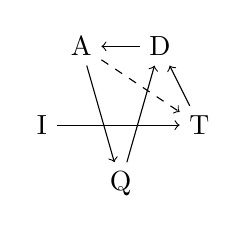
\begin{tikzpicture}
        \node[] at (-0.5,0.75) (a) {A};
        \node[] at (1,-0.25) (t) {T};
        \node[] at (0.5,0.75) (d) {D};
        \node[] at (-1,-0.25) (i) {I};
        \node[] at (0,-1) (q) {Q};
        \draw[->] (a) -- (q);
        \draw[dashed,->] (a) -- (t);
        \draw[->] (t) -- (d);
        \draw[->] (q) -- (d);
        \draw[->] (i) -- (t);
        \draw[->] (d) -- (a);
    \end{tikzpicture}
    \end{center}
    \item[Long:] consisted of a single syllable with a long vowel in Old Elvish. As with short affixes, iambic roots become trochaic, dactylic roots become anapaestic, anapaestic roots become quasi-trochaic or trochaic (under the same circumstances described above), \emph{but} trochaic and quasi-trochaic roots become iambic rather than dactylic.
    \begin{center}
        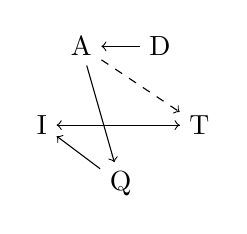
\begin{tikzpicture}
            \node[] at (-0.5,0.75) (a) {A};
            \node[] at (1,-0.25) (t) {T};
            \node[] at (0.5,0.75) (d) {D};
            \node[] at (-1,-0.25) (i) {I};
            \node[] at (0,-1) (q) {Q};
            \draw[->] (a) -- (q);
            \draw[dashed,->] (a) -- (t);
            \draw[->] (t) -- (i);
            \draw[->] (q) -- (i);
            \draw[->] (i) -- (t);
            \draw[->] (d) -- (a);
        \end{tikzpicture}
        \end{center}
    \item[Iambic:] consisted of two syllables, the latter with a long vowel and the former with a short vowel. Anapaestic roots become iambic, iambic roots become dactylic, dactylic roots become quasi-trochaic, and trochaic and quasi-trochaic roots remain trochaic and quasi-trochaic, respectively.
    \begin{center}
        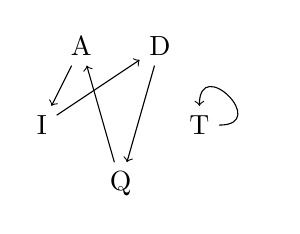
\begin{tikzpicture}
            \node[] at (-0.5,0.75) (a) {A};
            \node[] at (1,-0.25) (t) {T};
            \node[] at (0.5,0.75) (d) {D};
            \node[] at (-1,-0.25) (i) {I};
            \node[] at (0,-1) (q) {Q};
            \draw[->] (a) to (i);
            \draw[->] (t) to [out=0,in=90,loop,looseness=4.8] (t);
            \draw[->] (q) to (a);
            \draw[->] (i) to (d);
            \draw[->] (d) to (q);
        \end{tikzpicture}
    \end{center}
    \item[Trochaic:] consisted of two syllables, the latter with a short vowel and the former with a long vowel. Anapaestic roots become dactylic, dactylic roots become quasi-trochaic, quasi-trochaic roots become trochaic, and iambic and trochaic roots remain iambic and trochaic, respectively.
    \begin{center}
        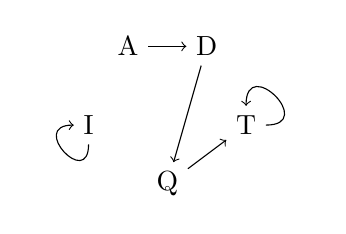
\begin{tikzpicture}
            \node[] at (-0.5,0.75) (a) {A};
            \node[] at (1,-0.25) (t) {T};
            \node[] at (0.5,0.75) (d) {D};
            \node[] at (-1,-0.25) (i) {I};
            \node[] at (0,-1) (q) {Q};
            \draw[->] (a) to (d);
            \draw[->] (t) to [out=0,in=90,loop,looseness=4.8] (t);
            \draw[->] (i) to [out=-90,in=180,loop,looseness=4.8] (i);
            \draw[->] (q) to (t);
            \draw[->] (d) to (q);
        \end{tikzpicture}
    \end{center}
    \item[Pyrrhic:] consisted of two syllables, both of which contained short vowels. Anapaestic and iambic roots become dactylic, dactylic roots become quasi-trochaic, quasi-trochaic roots become iambic, and trochaic roots remain trochaic.
    \begin{center}
        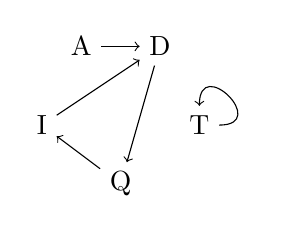
\begin{tikzpicture}
            \node[] at (-0.5,0.75) (a) {A};
            \node[] at (1,-0.25) (t) {T};
            \node[] at (0.5,0.75) (d) {D};
            \node[] at (-1,-0.25) (i) {I};
            \node[] at (0,-1) (q) {Q};
            \draw[->] (a) to (d);
            \draw[->] (t) to [out=0,in=90,loop,looseness=4.8] (t);
            \draw[->] (i) to (d);
            \draw[->] (q) to (i);
            \draw[->] (d) to (q);
        \end{tikzpicture}
    \end{center}
    \item[Anapaestic:] consisted of three syllables, the last of which was long with the prior two being short. Quasi-trochaic roots become trochaic, trochaic roots become dactylic, dactylic roots become iambic, iambic roots become anapaestic, and anapaestic roots remain anapaestic.
    \begin{center}
        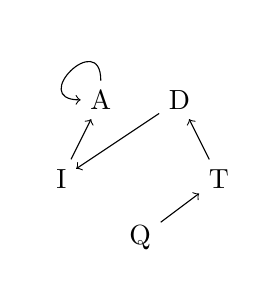
\begin{tikzpicture}
            \node[] at (-0.5,0.75) (a) {A};
            \node[] at (1,-0.25) (t) {T};
            \node[] at (0.5,0.75) (d) {D};
            \node[] at (-1,-0.25) (i) {I};
            \node[] at (0,-1) (q) {Q};
            \draw[->] (t) to (d);
            \draw[->] (a) to [out=90,in=180,loop,looseness=4.8] (a);
            \draw[->] (i) to (a);
            \draw[->] (q) to (t);
            \draw[->] (d) to (i);
        \end{tikzpicture}
    \end{center}
    \item[Amphibrachic:] consisted of three syllables, the middle of which was long with the other two being short. Dactylic roots remain dactylic. All other roots become or remain trochaic.
    \begin{center}
        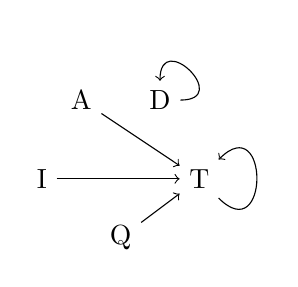
\begin{tikzpicture}
            \node[] at (-0.5,0.75) (a) {A};
            \node[] at (1,-0.25) (t) {T};
            \node[] at (0.5,0.75) (d) {D};
            \node[] at (-1,-0.25) (i) {I};
            \node[] at (0,-1) (q) {Q};
            \draw[->] (t) to [out=-45,in=45,loop,looseness=4.8] (t);
            \draw[->] (d) to [out=0,in=90,loop,looseness=4.8] (d);
            \draw[->] (i) to (t);
            \draw[->] (q) to (t);
            \draw[->] (a) to (t);
        \end{tikzpicture}
    \end{center}
    \item[Dactylic:] consisted of three syllables, the first of which was long with the other two being short. Anapaestic and iambic roots become trochaic. All other roots become or remain dactylic.
    \begin{center}
        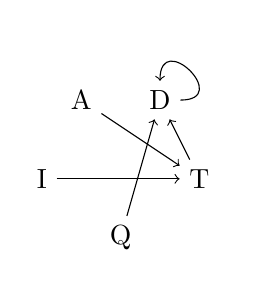
\begin{tikzpicture}
            \node[] at (-0.5,0.75) (a) {A};
            \node[] at (1,-0.25) (t) {T};
            \node[] at (0.5,0.75) (d) {D};
            \node[] at (-1,-0.25) (i) {I};
            \node[] at (0,-1) (q) {Q};
            \draw[->] (t) to (d);
            \draw[->] (d) to [out=0,in=90,loop,looseness=4.8] (d);
            \draw[->] (i) to (t);
            \draw[->] (q) to (d);
            \draw[->] (a) to (t);
        \end{tikzpicture}
    \end{center}
    \item[Cretic:] consisted of three syllables, the first and last of which were long and the middle of which was short. Iambic roots become trochaic, and anapaestic roots remain anapaestic. All other roots become iambic.
    \begin{center}
        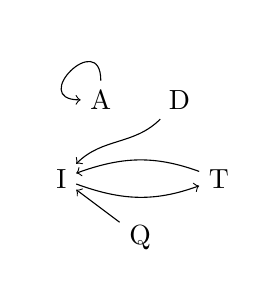
\begin{tikzpicture}
            \node[] at (-0.5,0.75) (a) {A};
            \node[] at (1,-0.25) (t) {T};
            \node[] at (0.5,0.75) (d) {D};
            \node[] at (-1,-0.25) (i) {I};
            \node[] at (0,-1) (q) {Q};
            \draw[->] (t) to [out=160,in=20] (i);
            \draw[->] (d) to [out=225,in=45] (i);
            \draw[->] (i) to [out=-20,in=200] (t);
            \draw[->] (q) to (i);
            \draw[->] (a) to [out=90,in=180,loop,looseness=4.8] (a);
        \end{tikzpicture}
    \end{center} 
\end{description}
While there may be some indicator of which category a given affix falls into based on how it patterns with roots, by and large these cannot be reliably inferred from surface forms without some knowledge of historical forms. Within this grammar, the underlying pattern of a given affix will be listed when relevant. 

Since affixes naturally appear differently in different environments, their differences will be listed when relevant. If in a context where pointing out each individual form is unnecessary or has already been done, the form used with anapaestic roots will be used as the citation form for nouns and the form used with dactylic roots will be used as the citation form for verbs.

\subsection{Historic glottals and vowels}

Sometimes a given affix form will be written out with a superscript \supho{} or \supglot{} preceding or following the affix. This indicates that in Old Elvish there was a historic \proto{h} or \proto{\glotstop} present at that boundary that could affect adjacent phones. Historically root-final vowels will have their tone raised prior to \supglot{} and lowered prior to \suph{}, as occurred in other contexts where these phones were historically present. Additionally, obstruents which were affected by adjacent glottals will also be affected by these historical glottals. For example, when the suffix \enl{-\supglot{}wạ} is placed after a vowel-final root like \enl{nala}, the form is realized as \enl{naláwạ}. If the same suffix is placed after a stop-final root like \enl{mak}, the form is realized as \enl{ma\kka wạ} (not \enl{makwạ}) due to the influence of the historic glottal on the final consonant.

If a historic final \proto{h} or \proto{\glotstop} preceded a historic short vowel that has since been deleted, that vowel will be incorporated into the superscript (as \supho{}, \supha{}, \suphi{}, \supgloto{},\supglota{}, \supgloti{}). When once of these precedes a morpheme that begins with a historic glottal, a glide is inserted at the place of articulation of the historic vowel. For example, the form of the inclusive subject clitic that is placed after a dactylic root is \enl{-mạ\supho}, an iambic affix that turns the root quasi-trochaic. The form of the exclusive object clitic that is placed directly after is \enl{-\supglot wạ}. Without these morpheme-boundary indicators, one would expect the form to be \enl{-mạwạ}, but due to their interactions, it's actually \enl{-mạwwạ}. Minor `irregularities' like this frequently result from these interactions, which is why these superscript indicators are included when relevant. 

Some morphemes (usually alternate forms of particular morphemes) will begin with a \supg{}. This is used to indicate the creation of a glide from the final historic short consonant in certain roots under certain circumstances (generally not including cases with historic glottals). These forms are rarer than historic glottals, as they only occur when a particular sound change was licensed, and as such the historic final vowel of roots without a historic final consonant is usually not listed (unless this particular affect is being illustrated). Instead, one must usually consult the etymology of the root in question if it appears before a morpheme with a \supg{} present.

\section{Nominal Morphology}

Nouns are obligatorily marked for number and a combination of specificity and definiteness, albeit in different ways. Number is marked through one of several affixes used to distinguish 3-5 grammatical numbers (the precise number depends on how you analyze them). Meanwhile, specificity and definiteness are attached via clitics attaching to the rightmost edge of the noun phrase. Both are obligatory and cannot be omitted.

\subsection{Number Marking}

Nouns in \parentlang{} generally fall into two classes, each of which displays different characteristics when it comes to marking of number. The two classes are generally called `singular' and `collective', as those are the number assumed to be present on the unmarked form of a given noun in that class. 

\begin{table}[htb]
    \centering
    \begin{tabular}{@{}rclllll@{}}
    \toprule
     & \textbf{Metre} & \multicolumn{1}{c}{\textbf{Iambic}} & \multicolumn{1}{c}{\textbf{Anapaestic}} & \multicolumn{1}{c}{\textbf{Dacylic}} & \multicolumn{1}{c}{\textbf{Trochaic}} & \multicolumn{1}{c}{\textbf{Quasi-trochaic}} \\\midrule
    \textbf{Paucal} & trochaic & \textit{-\supglot{}mo} & \textit{-\supglot{}m} & \textit{-\supglot{}ẹm} & \textit{-\supglot{}ẹm} & \textit{-\supglot{}ẹm} \\
    \textbf{Plural} & dactylic & \textit{-\supglot{}\ppa{}ip} & \textit{-\supglot{}\ppa{}ip} & \textit{-\supglot{}ị\ppa{}} & \textit{-\supglot{}ị\ppa{}} & \textit{-\supglot{}ị\ppa{}} \\\bottomrule
    \end{tabular}
    \caption{Nominal Number Suffixes}
    \label{tab:noun-num}
\end{table}

Singular nouns describe one entity (i.e., are singular) in their unmarked form. They generally describe things in which a singular individual can be discretely observed more often than not---for example, \enl{matí} `elf, person' (underlyingly \enl{matí\suphi{}} for purposes of morpheme boundary effects), is singular. In addition to the zero-marked singular number, there are two further delineations in number: \gls{pau} and \gls{pl}. The paucal is used for quantities of a noun that are greater than one but less than five. Unlike in languages with a binary singular-plural distinction, the plural in \parentlang{} is only used for quantities of at least five. So a group of four people would be described as \enl{matíyẹm}, whereas a group of five would be described as \enl{matíyị\ppa}

Collective nouns, roughly speaking, describe things that are generally discussed in multiples rather than as a single item. For instance, the words \enl{\tta{}ẹmo} `eyes' and \enl{í\ppa ạyạ} `almond flour' are collective, meaning that in their unmarked forms they refer to multiple items or a quantity of items. To refer to a single tree branch or a single grain of flour, one uses the \gls{sgv} marker \enl{yó-}, which explicitly picks out `one piece' from the group of objects a collective noun describes. For instance, if one needs to explicitly refer to a single eye, one uses the form \enl{yó\tta{}ẹmo}. 

The singulative marker is unusual in that it is a prefix, due to its originally having been a head noun used to form a compound. As a result, it can cause historical stress/length changes in the root it attaches to that form irregular singulative forms. For instance, the singulative form of \enl{í\ppa ạyạ} is \enl{yo\ppa\ppa ạyạ}, not \enl{yóí\ppa ạyạ}. These are explicitly indicated in dictionary entries, as there generally isn't a clear synchronic way to derive them consistently.

To emphatically describe a multitude of a given object, one can accompany the plural suffix with emphatic reduplication of the initial consonant (if any) and vowel of the word. This does not affect the metre of the word in any way. For example, in order to refer to a multitude of people, a speaker may say \enl{mamatíyị\ppa}. Unlike ordinary paucal and plural marking, this process is allowed for collective nouns, describing an incredibly large amount or quantity. For instance, a speaker could refer to a massive quantity of almond flour as \enl{íí\ppa ạya\ppa{}ip}. This is the only context in which collective nouns can take the marking ordinarily reserved for singular nouns.

\subsection{Definiteness \& Specificity}

Definiteness and specificity are marked by appending given clitics to the last element in a noun phrase. For bare nouns, this entails attachment to the noun itself, but for nouns modified by adjectives, the definiteness and specificity marking attaches to the rightmost element and thus to one of the adjectives. 

\begin{table}[htb]
    \centering
    \begin{tabular}{@{}rclllll@{}}
    \toprule
    \textit{\textbf{}} & \textbf{Metre} & \multicolumn{1}{c}{\textbf{Iambic}} & \multicolumn{1}{c}{\textbf{Anapaestic}} & \multicolumn{1}{c}{\textbf{Dactylic}} & \multicolumn{1}{c}{\textbf{Trochaic}} & \multicolumn{1}{c}{\textbf{Quasi-trochaic}} \\ \midrule
    \textbf{Specific} & iambic & \textit{-s\supho{}} & \textit{-só} & \textit{-si\supho{}} & \textit{-si\supho{}} & \textit{-só} \\
    \multicolumn{2}{r}{\textbf{+ definite}} & \textit{-sło} & \textit{-sół} & \textit{-sił} & \textit{-sił} & \textit{-sół} \\
    \textbf{Non-specific} & iambic & \textit{-\suph{}y\supho{}} & \textit{-\suph{}yó} & \textit{-\suph{}i\supho{}} & \textit{-\suph{}i\supho{}} & \textit{-\suph{}yó} \\
    \multicolumn{2}{r}{\textbf{+ definite}} & \textit{-\suph{}yło} & \textit{-\suph{}yół} & \textit{-\suph{}ił} & \textit{-\suph{}ił} & \textit{-\suph{}yół} \\ \bottomrule
    \end{tabular}
    \caption{Specificity \& Definiteness Clitics}
    \label{tab:spec-def}
\end{table}

Technically speaking, on a historical level, the specificity and definiteness markers are separate entities. However, since the definiteness marker never occurs without some specificity marker, it's more practical to display them all together in \autoref{tab:spec-def}.

In general, definiteness morphology serves to indicate that the speaker considers the referent in question to be uniquely identifiable to the hearer. Specific and non-specific indefinites can be distinguished in that specific indefinites refer to a particular indefinite individual (or set thereof) whereas non-specific ones refer to any member of a class of inidividuals. Nonspecific definites serve to mark what/whoever fills a particular identifiable role. More discussion of the precise semantics of these markers can be found in \autoref{sec:spec-def}

\subsection{Quantification}

While some degree of quantification is naturally described by nominal number marking, often the speaker wishes to express further quantification. In \parentlang{}, this is expressed through the addition of one of several quantificational clitics. As each of these clitics originates from the combination of two words from Old Elvish, each has two labels for metre, indicating the metre of each of the original two parts. 

\begin{table}[htb]
    \centering
    \begin{tabular}{@{}rclllll@{}}
        \toprule
        & \textbf{Metre} & \textbf{Iambic} & \textbf{Anapaestic} & \textbf{Dactylic} & \textbf{Trochaic} & \textbf{Quasi-trochaic}\\
        \textbf{Universal} & iambic + trochaic & \textit{-\kka\kka ẹn} & \textit{-\kka ánga} & \textit{-ka\kka ẹn} & \textit{-ka\kka ẹn} & \textit{\kka áng} \\
        \textbf{Negative} & trochaic + trochaic & \textit{-\suph{}sánga} & \textit{-\suph\tta ẹn} & \textit{-\suph{}ó\tta ẹn} & \textit{-\suph{}ó\tta ẹn} & \textit{-\suph{}ó\tta ẹn} \\
        \textbf{Partitive} & short + trochaic & \textit{-sẹn} & \textit{-sẹn} & \textit{-séng} & \textit{-sẹn} & \textit{-sẹn} \\
        \bottomrule
    \end{tabular}
    \caption{Quantificational Clitics}
    \label{tab:quant}
\end{table}

These clitics attach at the rightmost edge of the `quantificational phrase', consisting of the entire NP as well as any following overt numerals. If there is no overt numeral, the quantificational clitic attaches directly after the definiteness/specificity clitics, but if there is an overt numeral following these, it attaches to the numeral. For instance, `none of the elves' would be \enl{matíyẹmsó\l ó\tta ẹn} but `none of the three elves' would be \enl{matíyẹmsó\l{} séngạsánga}. More specific partitive quantities are expressed by the inclusion of another explicit numeral following the application of the partitive clitic---e.g., `two of the three elves' would be \enl{matíyẹmsó\l{} séngạsẹn poł}. This can be applied recursively until it reaches the limits of the speaker and hearer's ability to process the resulting phrase.

\section{Verbal Morphology}

\parentlang{} verbal morphology involves the use of affixes to mark tense as well as, in many contexts, using anaphoric clitics to indicate the person of verbal arguments. Tense affixes are mandatory and appear closest to the verb, whereas anaphoric clitics are only included in certain contexts and occur after any tense affix. Historically \parentlang{} possessed a negation affix that occurred even closer to the verb stem than tense marking; however, as negation is now largely indicated analytically, this is only apparent in the derivations of negation particles from \parentlang{} verbs.

\subsection{Tense Marking}

\parentlang{} obligatory tense marking makes a present vs. nonpresent disctinction, with five degrees of remoteness in nonpresent forms. Present tense is unmarked/null, whereas the other tenses have the following forms:

\begin{table}[h]
    \centering
    \begin{tabular}{@{}rclllll@{}}
        \toprule
        \textbf{} & \textbf{Metre} & \multicolumn{1}{c}{\textbf{Iambic}} & \multicolumn{1}{c}{\textbf{Anapaestic}} & \multicolumn{1}{c}{\textbf{Dactylic}} & \multicolumn{1}{c}{\textbf{Trochaic}} & \multicolumn{1}{c}{\textbf{Quasi-trochaic}} \\ \midrule
        \textbf{Immediate} & pyrrhic & \textit{-syan} & \textit{-syan} & \textit{-sén} & \textit{-sén} & \textit{-sna} \\
        \textbf{Near} & long & \textit{-k} & \textit{-k} & \textit{-ko} & \textit{-ko} & \textit{-ko} \\
        \textbf{Medial} & short & \textit{-ng} & \textit{-ng} & \textit{-ngo} & \textit{-ng} & \textit{-ng} \\
        \textbf{Far} & trochaic & \textit{-tmo} & \textit{-tyom} & \textit{-tem} & \textit{-tem} & \textit{-tem} \\
        \textbf{Mythic} & cretic & \textit{-\supglot{}rạ\suphi{}} & \textit{-\supglot{}rrí} & \textit{-\supglot{}arí} & \textit{-\supglot{}arí} & \textit{-\supglot{}arí} \\ \bottomrule
        \end{tabular}
    \caption{Tense Morphemes}
    \label{tab:tense-morph}
    \end{table}

A general explanation of these tenses is that the unmarked present tense indicates that an eventuality occurs or is ongoing at the utterance time, while the various non-present tenses indicate various degrees of removal from the utterance time in either direction. The immediate tense emphasizes the closeness of the eventuality to the present, with the event occurring immediately before or after the utterance time. The near tense indicates something occurring within a fairly short period, the medial tense within a slightly longer period, the far tense within an even longer period, and the mythic tense is used for things that occur at times extremely far removed from the present. The finer semantic details of these tenses discussed in \autoref{sec:tense}.

\subsection{Anaphoric Clitics}\label{subsec:morph_ana_clit}

Both the subject and object of a verb in \parentlang{} can be marked with anaphoric clitics if they aren't expressed by overt noun phrase arguments in the sentence proper. Unlike agreement markers, these anaphoric clitics only appear when there aren't overt noun phrase arguments---they appear when another langauge might use a pronominal argument. Note that these are not used for focused pronominal arguments or pronouns that are otherwise emphasized---there are distinct, analytic pronominal forms that are used in those circumstances. These clitics are instead used in contexts in which a pro-drop language would likely drop the relevant pronominal form entirely.

\begin{table}[htb]
    \centering
    \begin{tabular}{@{}crclllll@{}}
    \toprule
     &  & \textbf{Metre} & \multicolumn{1}{c}{\textbf{Iambic}} & \multicolumn{1}{c}{\textbf{Anapaestic}} & \multicolumn{1}{c}{\textbf{Dactylic}} & \multicolumn{1}{c}{\textbf{Trochaic}} & \multicolumn{1}{c}{\textbf{Quasi-Trochaic}} \\ \midrule
    \multirow{4}{*}{\rotatebox[origin=c]{90}{\textbf{Subject}}} & \Excl{}\Actson & trochaic & \textit{-\suph{}ma} & \textit{-\suph{}m} & \textit{-\suph{}ám} & \textit{-\suph{}ám} & \textit{-\suph{}ám} \\
     & \Incl{}\Actson & iambic & \textit{-m\supho{}} & \textit{-mó} & \textit{-mạ\supho{}} & \textit{-mạ\supho{}} & \textit{-mó} \\
     & \Second{}\Actson & iambic & \textit{-f\supho{}} & \textit{-fó} & \textit{-fo\supho{}} & \textit{-fo\supho{}} & \textit{-fó} \\
     & \Third{}\Actson & pyrrhic & \textit{-\suph{}w\supgloti{}} & \textit{-\suph{}w\supgloti{}} & \textit{-\suph{}ó\supgloti{}} & \textit{-\suph{}ó\supgloti{}} & \textit{-\suph{}wị} \\ \midrule
    \multirow{4}{*}{\rotatebox[origin=c]{90}{\textbf{Object}}} & \ToExcl & iambic & \textit{-\supglot{}w\supglota{}} & \textit{-\supglot{}wạ} & \textit{-\supglot{}o\supglota{}} & \textit{-\supglot{}o\supglota{}} & \textit{-\supglot{}wạ} \\
     & \ToIncl & iambic & \textit{-\kka} & \textit{-\kka ạ} & \textit{-kí\supglota{}} & \textit{-kí\supglota{}} & \textit{-\kka ạ} \\
     & \ToSecond & long & \textit{-k} & \textit{-k} & \textit{-ki} & \textit{-ki} & \textit{-ki} \\
     & \ToThird & short & \textit{-\l} & \textit{-\l} & \textit{-\l o} & \textit{-\l} & \textit{-\l} \\ \bottomrule
    \end{tabular}
\caption{Anaphoric Clitic Forms}
\label{tab:anaphoric-clitics}
\end{table}

Four different persons are distinguished in \parentlang{}---\gls{excl}, \gls{incl}, \gls{second}, and \gls{third} based on whether they refer to the speaker, hearer, both, or neither. These forms are used regardless of number; only the presence or absence of the speaker and hearer from a group is taken into account. The forms for each of these, for both the subject and the object, are illustrated in \autoref{tab:anaphoric-clitics}. As these clitics attach after the tense affixes, they attach based on the verb's metre \emph{after} it has been affected by the metre of any tense affix attached to the verb. The object clitics additionally attached after the subject clitics when both are present and are thus further affected by any changes to the metre effected by the subject clitics.


\chapter{Syntax}

\begin{figure}[htb]
    \centering
    \begin{tikzpicture}
        \Tree [.CP ContrFoc [.C' [.C C \node(t2){T}; ] [.TP Top [.T' [.\node(t){T}; T \node(v2){V}; ] [.VP NP [.V' [.\node(v){V}; V \edge[dashed]; {Adv} ] NP ] ] ] ] ] ]
        \draw[->,dashed] (v).. controls +(west:1) and +(south:1)..(v2);
        \draw[->,dashed] (t).. controls +(west:1) and +(south:1)..(t2);
    \end{tikzpicture}
    \caption{Basic structure of the \parentlang{} syntax}
    \label{fig:syntaxtree}
\end{figure}

\section{Underlying Word Order}

\parentlang{} syntax is largely head-initial and is highly discourse-configurational, with the syntax prioritizing the notions of topic and focus over the notions of subject and object when it comes to constituents' positions in the syntax and any movement operations applied to them. 

Even the underlying configuration of the verb and arguments prior to any movement, which could be superficially called SVO, is in fact not dependent on which argument is more agent-like or more patient-like, but rather on how salient/given they are in the discourse. The argument that has more clearly established itself in the common ground, be it through being previously mentioned or through being more salient in the discourse context, inhabits the `subject' slot, and the argument that is less suitable for this position takes the `object' position. This, of course, is only relevant for transitive verbs, as the single argument of an intransitive verb is necessarily the most salient/given of the verb's arguments. Since the traditional syntactic subject is more often the more salient of a verb's two arguments, `subject' and `object' will be used for the higher and lower argument respectively for the sake of having the simplest possible terminology, but it's certainly worth noting that the distinction here is closer to the prototypical proximate-obviate distinction than it is to the protoypical distinction between syntactic subject and object.

Note that this is not true of the use of `subject' and `object' in terms of the anaphoric clitics mentioned in \autoref{subsec:morph_ana_clit}, which do correspond to the more traditional morphosyntactic alignment that is expressed through the morphology. The references above refer solely to the use of these terms in reference to the underlying word order.

\subsection{Head Movement}

\section{Syntax-Discourse Interface}

\subsection{Topic Marking}

\subsection{Focus Marking}

\chapter{Semantics}

\section{Definiteness \& Specificity}\label{sec:spec-def}

\section{Tense \& Stuff}\label{sec:tense}

%\part{\childlangone{} Grammar}

%\chapter{Context \& Culture}

%\chapter{Phonology}

%Daughterlang ideas to save for later:

% \begin{itemize}
%     \item \phipa{lw, \vell w} become \bripa{\alvr\lab, \velr\lab}
% \end{itemize}

% \subsection{Romanization}

% \chapter{Morphosyntax}

% \chapter{Semantics}

\part{Dictionary}

\setsecnumdepth{part}
\settocdepth{part}

\chapter{Old Elvish}

\begin{multicols*}{2}

\begin{entrylist}
    \begin{protentry}{hi\lgth lino}\label{OE:hiilino}
        \dictdef*{
            speech, talking, discussion, chatting, communication\\
            {\footnotesize Descendants: 
            \textit{\nameref{enl:enLalen_HLM}}
            }
        }
    \end{protentry}
    \begin{protentry}{hi\lgth na\glotstop ala\lgth}
    \label{OE:hiina7alaa}
        \dictdef*{
            the World, the physical realm, the mortal plane, this world\\
            {\footnotesize Descendants: 
            \textit{\nameref{enl:enLalen_HLM}}
            }
        }
    \end{protentry}
\end{entrylist}

\end{multicols*}

\chapter{En\l alen}

\begin{multicols*}{2}

\section{E}

\begin{entrylist}
    \begin{dictentry}[ẽ\engma\toneH\vell a\toneL lẽn\toneM]{énłạlen}{
        troch., from Old Elv. \proto{hi\lgth na\glotstop ala\lgth hili\lgth no} `World-speech' from \proto{\nameref{OE:hiina7alaa}} `the World' + \proto{\nameref{OE:hiilino}} `speech'
        }
        \label{enl:enLalen_HLM}
        \dictdef*[n.]{this language, En\l alen}
    \end{dictentry}
\end{entrylist}

\section{I}

\begin{entrylist}
    \begin{dictentry}[il\toneH jũn\toneM]{ílyon}{
        dacty., from Old Elv. \proto{\nameref{OE:hiilino}} `speech'
    }
        \dictdef*[v.]{
            utterance, statement, sentence
        }
        \begin{entrysublist}
            \begin{simplentry}{ẹn ílyon}
                \dictdef*[v.]{
                    to be sapient, to be intelligent, to be mentally aware, to have one's faculties (lit., to have speech)
                }
            \end{simplentry}
        \end{entrysublist}
    \end{dictentry}
\end{entrylist}

\end{multicols*}

\part{Texts \& Translations}

%\backmatter

\end{document}